%=====================================================================
% 5  曲线模空间的欧拉示性数
% 原文：Section 5. The Euler characteristic of the moduli space of curves
%       （arXiv:2409.03117v1, p. 63--74）
%=====================================================================
\section{曲线模空间的欧拉示性数}

\begin{keytakeaways}
\begin{itemize}
  \item \textbf{物理图像：}矩阵积分（特别是相关多项式的计算）不仅能给出多边形粘合数，还能进一步算出曲线模空间的轨形欧拉示性数；这正是 Harer 与 Zagier 在 1986 年完成的经典工作。
  \item \textbf{数学工具：}Wall 意义下的群欧拉示性数（有限群的取值为群阶的倒数）、轨形欧拉示性数、Quillen 的胞腔求和公式，以及 Mumford 关于 Teichmüller 空间组合模型的定理。
  \item \textbf{关键结论：}带一个标记点的曲线模空间，其轨形欧拉示性数等于 $-\frac{B_{2{\rm g}}}{2{\rm g}}$；不带标记点时则为 $\frac{B_{2{\rm g}}}{4{\rm g}({\rm g}-1)}$。
  \item \textbf{证明策略：}把填满弧系的计数化为“带限制的多边形粘合计数”，利用三种粘合计数（不加条件、满足条件 (A)、满足条件 (A)、(B)）之间的二项式卷积关系与生成函数，把所求之和化为 欧拉 Beta 积分，最后由 $\Gamma'/\Gamma$ 的 Stirling 渐近展开读出 Bernoulli 数。
  \item \textbf{易错点：}Quillen 公式按 $(-1)^{\dim\sigma}/|{\rm Stab}\,\sigma|$ 加权；Poincaré 对偶胞腔的维数为 $6{\rm g}-3-n$，故符号恰为 $(-1)^{n-1}$，这是本章最容易弄错符号之处。
\end{itemize}
\end{keytakeaways}

\bigskip
\noindent\rule{\textwidth}{0.6pt}
\bigskip

矩阵积分（特别是多项式 $P_m(x)$ 的计算）可用于计算曲线模空间的轨形欧拉示性数。这一工作由 Harer 与 Zagier 于 1986 年完成。本节我们回顾这一结果（有所省略）。

\subsection{群的欧拉示性数}

我们首先回顾代数拓扑中的一些基本概念。

设 $\Gamma$ 为离散群，$Y$ 为可缩的有限维 CW 复形，$\Gamma$ 在其上作胞腔作用。这指的是 $\Gamma$ 通过 $Y$ 的同胚作用，且把每个胞腔同胚地映到另一个胞腔。我们假定每个胞腔的稳定子都是有限群（亦即 $Y$ 是真 $\Gamma$-复形，proper $\Gamma$-complex）。

先设 $\Gamma$ 的作用是自由的（即胞腔的稳定子平凡）。这等价于说 $\Gamma$ 是无挠的（torsion free，即没有非平凡有限子群），因为有限群不可能无不动点地作用在可缩的有限维胞腔复形上（它的上同调维数是无限的）。

此时可以定义胞腔复形 $Y/\Gamma$（$\Gamma$ 的分类空间），并且对任意系数群 $A$ 有 $H^i(Y/\Gamma,A)=H^i(\Gamma,A)$。特别地，若 $Y/\Gamma$ 有限，则 $\Gamma$ 的上同调维数有限，且欧拉示性数 $\chi(\Gamma):=\sum_i (-1)^i\dim H^i(\Gamma,\Bbb Q)$ 等于 $\sum_i (-1)^in_i(Y/\Gamma)$，其中 $n_i(Y/\Gamma)$ 表示 $Y/\Gamma$ 中 $i$ 维胞腔的个数。

然而这一设定限制很强，因为它只允许上同调维数有限的群，特别地排除了所有非平凡的有限群。因此我们考虑更一般的设定：假定某个有限指数子群 $\Gamma'\subset \Gamma$（而非 $\Gamma$ 本身）满足上述条件。此时可以定义 $\Gamma$ 的 Wall 意义下的欧拉示性数，即有理数 $[\Gamma:\Gamma']^{-1}\chi(\Gamma')$。

容易验证，Wall 意义下的欧拉示性数可用下述 \emph{Quillen 公式} 计算：
$$
\chi(\Gamma)=\sum_{\sigma\in {\rm cells(Y)}/\Gamma}\frac{(-1)^{\dim
    \sigma}}{|{\rm Stab}\sigma|}.
$$
特别地，这个数与 $\Gamma'$ 的选取无关（这一点也容易直接验证）。

% [Tutor Note: 有限群情形的 $\chi(G)=|G|^{-1}$ 是理解“加权”的关键：取有限指数子群为平凡群，并把 $Y$ 取为单点、$G$ 平凡地作用其上，于是 Quillen 公式中只剩一个 0 维胞腔轨道，其稳定子为整个 $G$，贡献为 $1/|G|$。这正是轨形欧拉示性数按 $1/|{\rm Aut}(x)|$ 加权的来源，与通常的拓扑欧拉示性数（例如 $H/SL_2(\Bbb Z)\cong\Bbb C$ 的 $\chi=1$）截然不同，切勿混用。以上解释只是形式说明，此时作用并不自由。]
\begin{example} 若 $G$ 是有限群，则 $\chi(G)=|G|^{-1}$（取平凡群作为有限指数子群）。
\end{example}

\begin{example} $G=SL_2(\Bbb Z)$。该群含有一个指数为 12 的子群 $F$，它是由两个生成元生成的自由群（请自行验证！）。群 $F$ 的欧拉示性数为 $-1$，因为其分类空间 $Y/F$ 是“8”字形（亦即 $Y$ 是“8”字形的万有覆盖）。因此 $SL_2(\Bbb Z)$ 的欧拉示性数为 $-\frac{1}{12}$。
\end{example}

Wall 意义下的欧拉示性数在轨形框架下有几何解释。具体地说，设 $\Gamma$ 如上（即 $\chi(\Gamma)$ 是定义良好的有理数），$M$ 是可缩流形，$\Gamma$ 在其上自由且真不连续地作用。此时点的稳定子有限，故 $M/\Gamma$ 是轨形。特别地，这意味着每一点 $x\in M/\Gamma$ 都附有一个有限群 ${\rm Aut}(x)$，其阶 $\le [\Gamma:\Gamma']$。设 $X_m$ 为 $M/\Gamma$ 中由自同构群 ${\rm Aut}(x)$ 的阶等于 $m$ 的那些点 $x$ 组成的子集。常常出现 $X_m$ 具有有限胞腔复形的同伦型的情形。此时，$M/\Gamma$ 的\emph{轨形欧拉示性数}定义为
$$
\chi_{\rm orb}(M/\Gamma)=\sum_m\frac{\chi(X_m)}{m}.
$$

现在断言 $\chi_{\rm orb}(M/\Gamma)=\chi(\Gamma)$。事实上，考察投影 $M/\Gamma'\to M/\Gamma$，容易看出 $\chi_{\rm  orb}(M/\Gamma)=\frac{1}{[\Gamma:\Gamma']}\chi(M/\Gamma')$。但 $M/\Gamma'$ 是 $\Gamma'$ 的分类空间，故 $\chi(M/\Gamma')=\chi(\Gamma')$，由此即得断言。

\begin{example} 考虑群 $\Gamma=SL_2(\Bbb Z)$ 作用在上半平面 $H$ 上。此时 $H/\Gamma$ 是椭圆曲线的模空间。作为拓扑空间它是 $\Bbb C$，其中所有点的自同构群都是 $\Bbb Z/2$，例外的是点 $i$（自同构群为 $\Bbb Z/4$）以及 $\rho=\frac{-1+i\sqrt{3}}{2}$（自同构群为 $\Bbb Z/6$）。因此 $H/\Gamma$ 的轨形欧拉示性数为 $(-1)\frac{1}{2}+\frac{1}{4}+\frac{1}{6}=-\frac{1}{12}$。这并不奇怪，因为我们已经证明 $\chi_{\rm orb}(H/\Gamma)=\chi(\Gamma)$，而后者算得为 $-\frac{1}{12}$。
\end{example}

\subsection{映射类群}

设 ${\rm g}\ge 1$ 为整数，$\Sigma$ 是亏格为 ${\rm g}$ 的闭可定向曲面。取 $p\in \Sigma$，并令 $\Gamma_{\rm g}^1$ 为保持 $p$ 的 $\Sigma$ 的微分同胚的同痕类（isotopy class）构成的群。我们依照 Harer 与 Zagier 的文章 \cite{HZ}，不加证明地回顾关于该群的一些标准事实。

群 $\Gamma_{\rm g}^1$ 并非无挠，但它含有一个有限指数的无挠子群。具体而言，考虑由 $\Gamma_{\rm g}^1$ 在 $H_1(\Sigma,\Bbb Z/n\Bbb Z)$ 上的作用给出的同态 $\Gamma_{\rm g}^1\to {\rm Sp}(2{\rm g},\Bbb Z/n\Bbb Z)$。则当 $n$ 充分大时（事实上 $n\ge 3$），该映射的核 $K_n$ 是无挠的。

结果表明，存在一个可缩的有限维胞腔复形 $Y_{\rm g}$（将在下文构造），$\Gamma_{\rm g}^1$ 在其上作胞腔作用，且只有有限多个胞腔轨道。因此 $\Gamma_{\rm g}^1$ 的 Wall 意义下的欧拉示性数是定义良好的。

\subsection{Harer–Zagier 定理}

$\Gamma_{\rm g}^1$ 的欧拉示性数由下述定理给出。

\begin{theorem} \label{hz}（Harer–Zagier）有
$$
\chi(\Gamma_{\rm g}^1)=-\frac{B_{2{\rm g}}}{2{\rm g}},
$$
其中 $B_n$ 是 Bernoulli 数。
\end{theorem}

\begin{remark} 群 $\Gamma_{\rm g}^1$ 作用在 Teichmüller 空间 ${\mathcal T}_{\rm g}^1$ 上；按定义，后者是所有二元组 $((R,z),f)$ 构成的空间，其中 $(R,z)$ 是带标记点 $z$ 的复 Riemann 曲面，而 $f$ 是微分同胚 $R\to \Sigma$ 的同痕类，且把 $z$ 映到 $p$。可以证明 ${\mathcal T}_{\rm g}^1$ 是维数为 $6{\rm g}-4$ 的可缩流形，且 $\Gamma_{\rm g}^1$ 在 ${\mathcal T}_{\rm g}^1$ 上的作用是真不连续的。特别地，可以定义轨形 $M_{\rm g}^1={\mathcal T}_{\rm g}^1/\Gamma_{\rm g}^1$。该轨形参数化上述二元组 $(R,z)$，因此称为亏格为 ${\rm g}$、带一个标记点的 Riemann 曲面（即光滑复射影代数曲线）的模空间。于是定理 \ref{hz} 给出了亏格为 ${\rm g}$、带一个标记点的曲线模空间的轨形欧拉示性数。
\end{remark}

\begin{remark} 若 ${\rm g}>1$，可以定义上述对象不带标记点的类似物，即映射类群 $\Gamma_{\rm g}$、Teichmüller 空间 ${\mathcal T}_{\rm g}$ 与曲线模空间 $M_{\rm g}={\mathcal T}_g/\Gamma_g$（对 ${\rm g}=1$ 也可同样定义，但此时与带一个标记点的情形没有区别，因为平移群可以把 $\Sigma$ 上任意两点等同起来）。容易看出，当 ${\rm g}>1$ 时有正合列 $1\to \pi_1(\Sigma)\to \Gamma_{\rm g}^1\to \Gamma_{\rm g}\to 1$，由此可得 $\chi(\Gamma_{\rm g})=\chi(\Gamma_{\rm g}^1)/\chi(\Sigma)$。因此 Harer–Zagier 定理给出 $\chi(\Gamma_{\rm g})=\chi_{\rm orb}(M_{\rm g})=\frac{B_{2{\rm g}}}{4{\rm g}({\rm g}-1)}$。
\end{remark}

% [Tutor Note: 由正合列 $1\to\pi_1(\Sigma)\to\Gamma_{\rm g}^1\to\Gamma_{\rm g}\to 1$ 得到 $\chi(\Gamma_{\rm g})=\chi(\Gamma_{\rm g}^1)/\chi(\Sigma)$，用的是群扩张（纤维化）的欧拉示性数乘性 $\chi(\Gamma_{\rm g}^1)=\chi(\pi_1(\Sigma))\,\chi(\Gamma_{\rm g})$，其中 $\chi(\pi_1(\Sigma))=2-2{\rm g}$；不要与有限指数子群的公式 $\chi(\Gamma')=[\Gamma:\Gamma']\chi(\Gamma)$ 混淆（两者是不同层面的乘性）。代入 Harer–Zagier 公式：$-B_{2{\rm g}}/(2{\rm g})$ 除以 $2-2{\rm g}$ 恰得 $B_{2{\rm g}}/(4{\rm g}({\rm g}-1))$。注意 ${\rm g}=1$ 时 $\chi(\Sigma)=0$，公式分母 $4{\rm g}({\rm g}-1)$ 退化，正因如此第二个注只对 ${\rm g}>1$ 陈述。]

\subsection{复形 $Y_{\rm g}$ 的构造}

我们从复形 $Y_{\rm g}$ 的构造开始证明定理 \ref{hz}，仍依循 \cite{HZ}。先构造一个带 $\Gamma_{\rm g}^1$ 作用的单纯复形，再用它构造 $Y_{\rm g}$。

设 $(\alpha_1,...,\alpha_n)$ 是 $\Sigma$ 上的一族闭简单无向曲线，它们均以 $p$ 为起点与终点，且除 $p$ 外互不相交。若满足下列两个条件，则称这样的族为\emph{弧系}（arc system）：

(A) 任何一条曲线都不能收缩为一点；

(B) 任何一条曲线都不能收缩为另一条曲线。

定义单纯复形 $A$：其 $n-1$ 维单形是含 $n\ge 1$ 条弧的弧系的同痕类；对应于 $(\alpha_1,...\alpha_n)$ 的单形的边界，是对应于弧系 $(\alpha_1,...,\widehat\alpha_i,...,\alpha_n)$（即删去 $\alpha_i$）的各单形之并。

显然，群 $\Gamma_{\rm g}^1$ 在 $A$ 上作单纯作用。

\begin{example} 取 ${\rm g}=1$，即 $\Sigma=S^1\times S^1$。此时 $\Gamma_{\rm g}^1=SL_2(\Bbb Z)$。模去它的作用，只有三个弧系（图 15）。具体地说，把 $S^1$ 视为复平面中的单位圆并用参数表示弧，可把这三种弧系写成：
$$
B_0=\lbrace{(e^{i\theta},1)\rbrace}; B_1=
\lbrace{(e^{i\theta},1),(1,e^{i\theta})\rbrace};
B_2=\lbrace{(e^{i\theta},1),(1,e^{i\theta}),(e^{i\theta},e^{i\theta})\rbrace}
$$
由此容易求出单纯复形 $A$。具体地说，设 $T$ 是以 $t_0$ 为根、与三个顶点 $t_1,t_2,t_3$ 相连的树：每个 $t_i$ 又与两个顶点 $t_{i1},t_{i2}$ 相连，每个 $t_{ij}$ 再与 $t_{ij1},t_{ij2}$ 相连，如此继续（图 16）。在 $T$ 的每个顶点处放一个三角形，使其边横截于由该顶点出发的三条棱，再把这些三角形沿它们的边粘合起来。这样得到的复形就是 $A$，见图 17（请自行验证！）。$SL_2(\Bbb Z)$（更确切地说 $PSL_2(\Bbb Z)$）在该复形上的作用容易描述。具体地说，回忆 $PSL_2(\Bbb Z)$ 由 $S,U$ 生成，定义关系为 $S^2=U^3=1$。$S,U$ 在 $T$ 上的作用如下：$S$ 是关于以 $t_0$ 为中心的三角形 $\Delta_0$ 的一条边的带翻转的反射（图 18），$U$ 是绕 $t_0$ 的 $2\pi/3$ 旋转。
\end{example}

\begin{figure}[htbp]
  \centering
  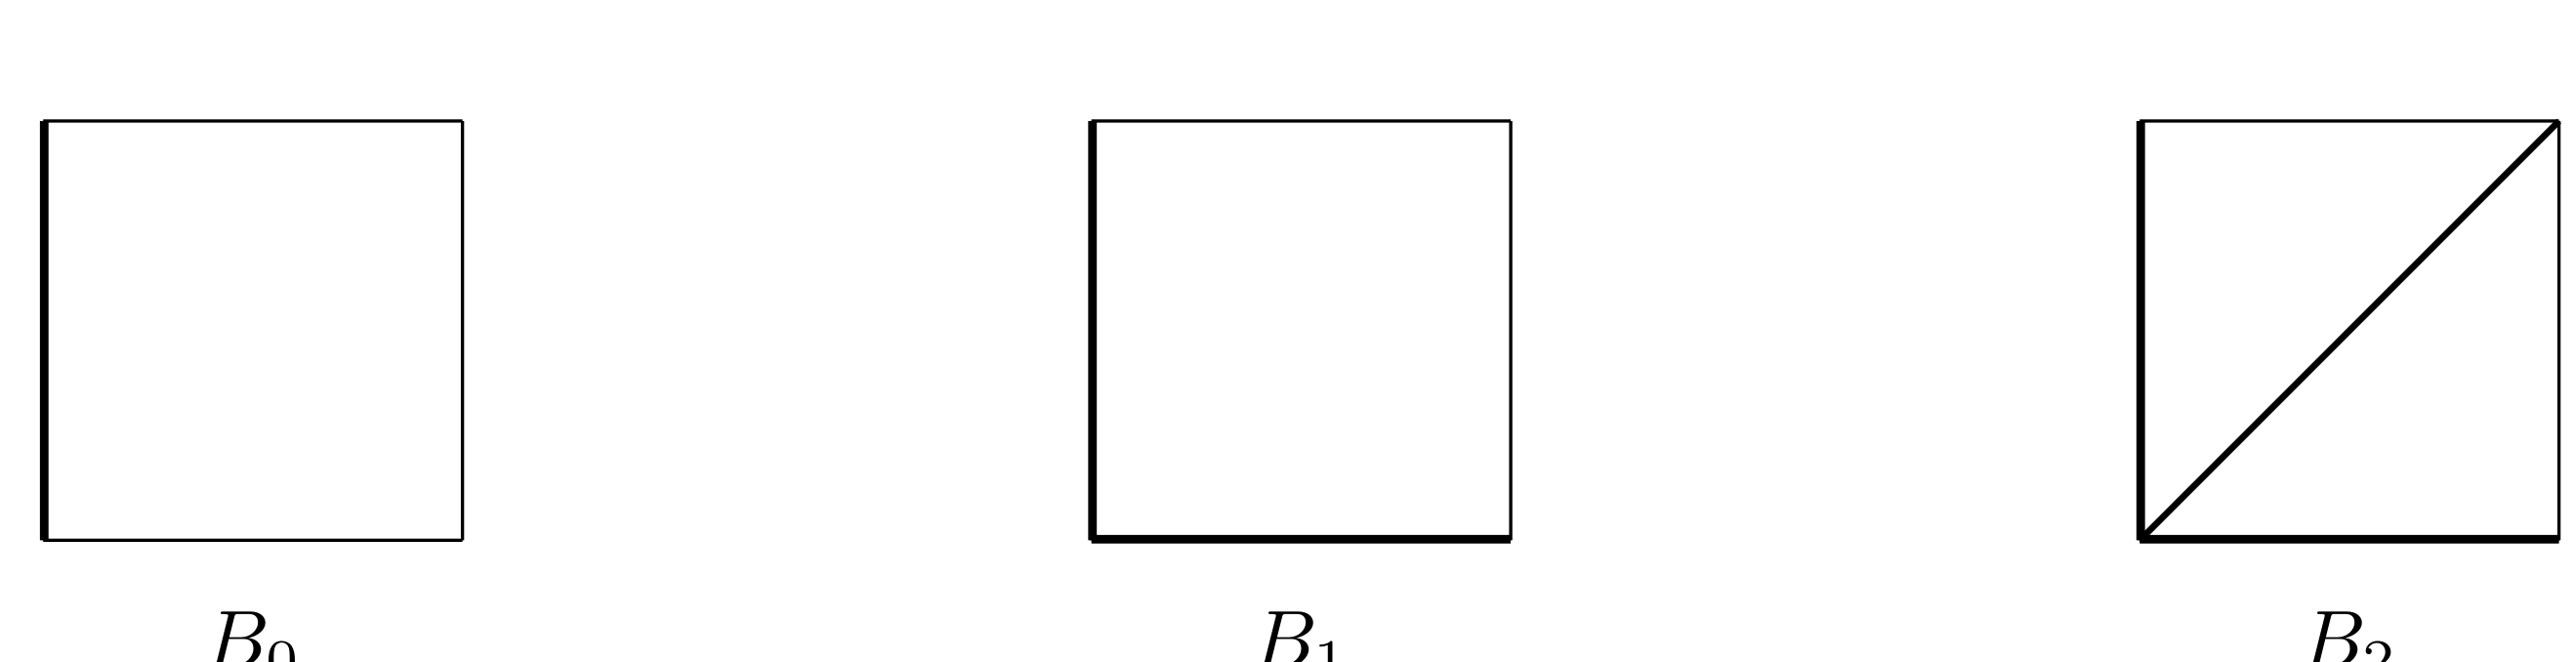
\includegraphics[width=11.16cm]{figures/fig-15.png}
  \caption{三个弧系。\figorig{67}{15}}
  \label{fig:15}
\end{figure}



\begin{figure}[htbp]
  \centering
  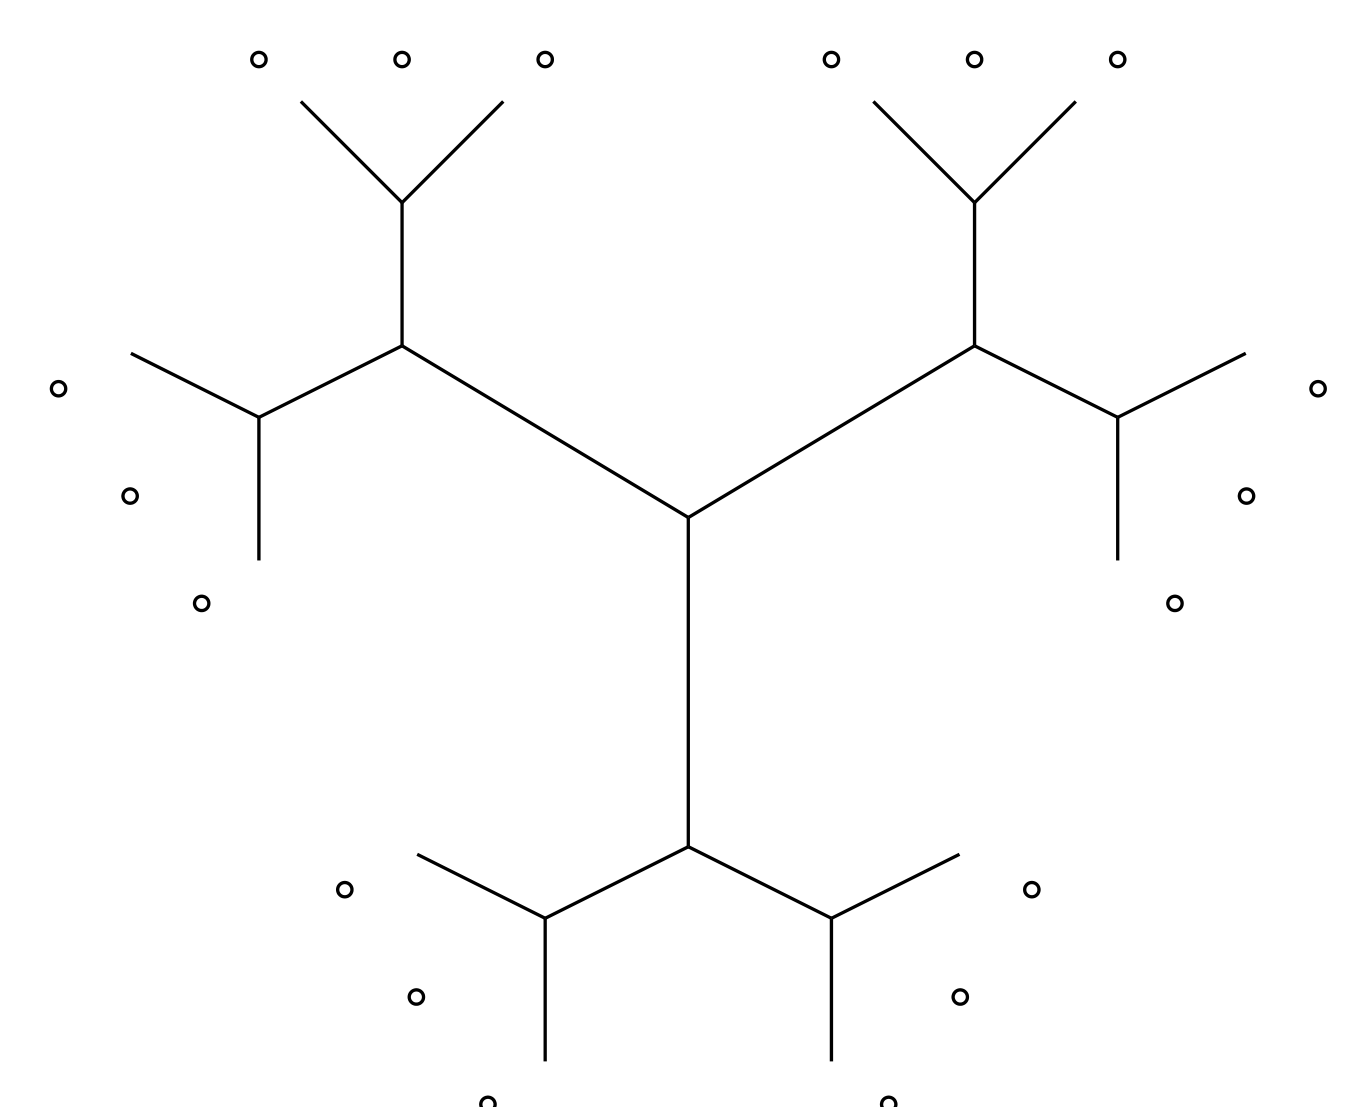
\includegraphics[width=5.71cm]{figures/fig-16.png}
  \caption{树 $T$\figorig{67}{16}}
  \label{fig:16}
\end{figure}


\begin{figure}[htbp]
  \centering
  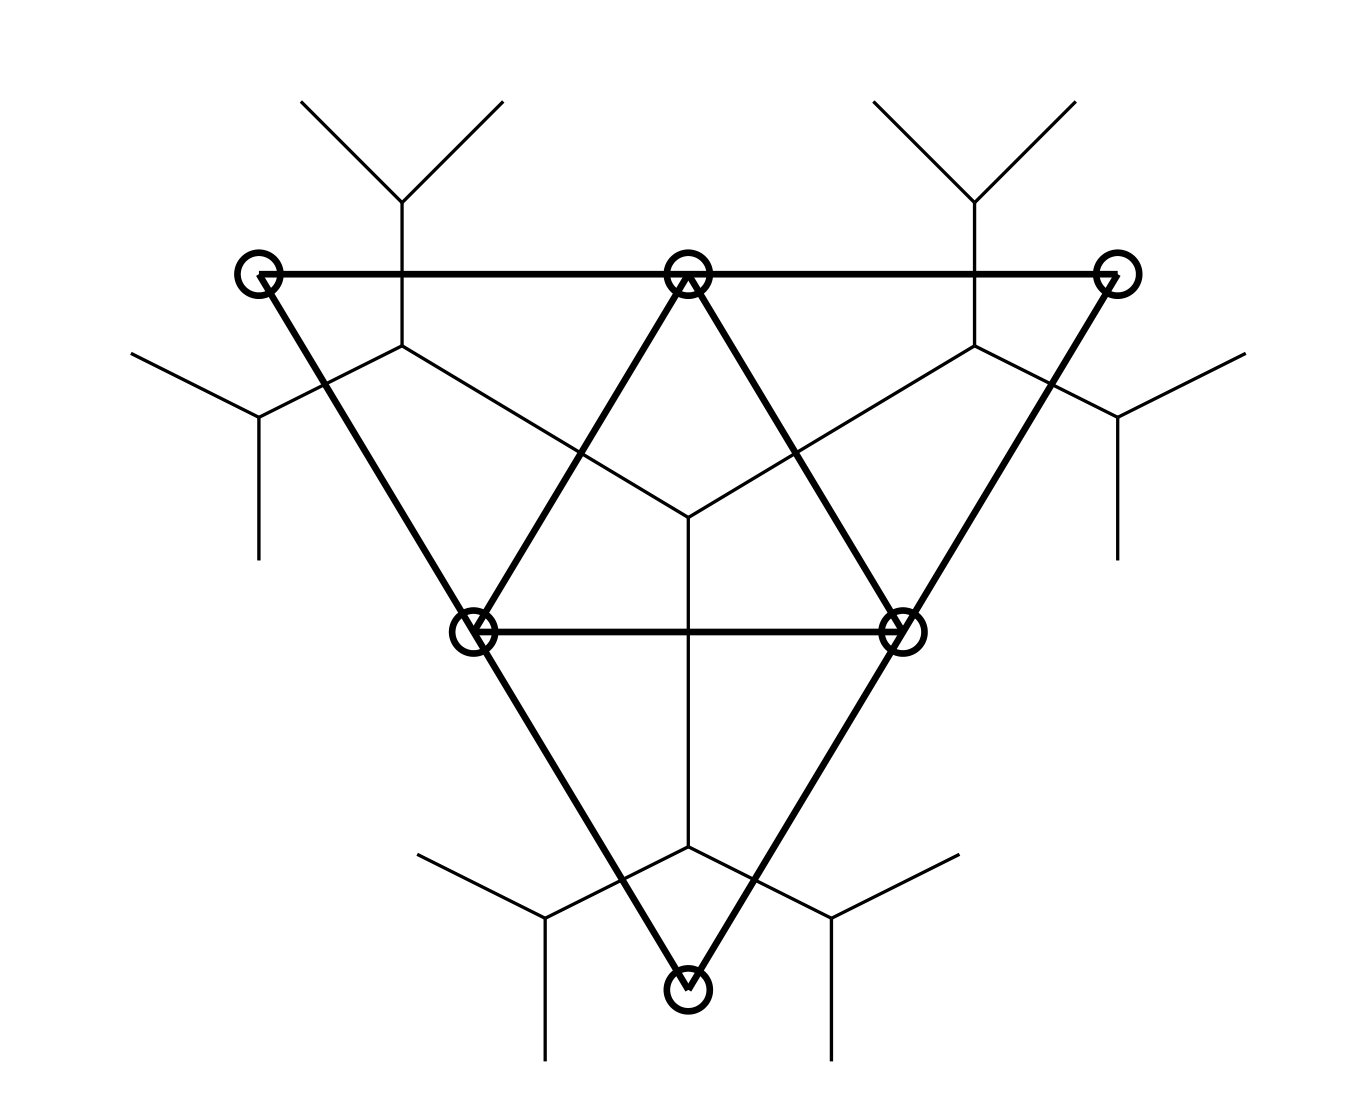
\includegraphics[width=5.71cm]{figures/fig-17.png}
  \caption{复形 A\figorig{68}{17}}
  \label{fig:17}
\end{figure}


\begin{figure}[htbp]
  \centering
  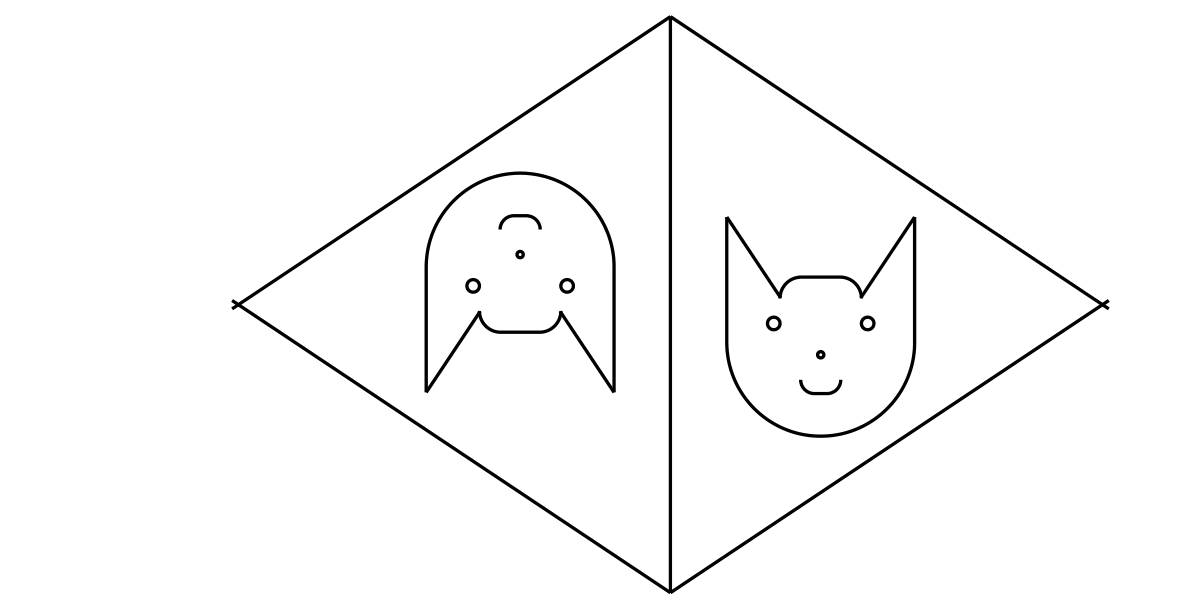
\includegraphics[width=5.03cm]{figures/fig-18.png}
  \caption{带翻转的反射。\figorig{68}{18}}
  \label{fig:18}
\end{figure}


这一例子表明，$\Gamma_{\rm g}^1$ 在 $A$ 上的作用并非真不连续，因为某些单形具有无限稳定子（在上例中就是 0 维单形）。因此我们希望丢掉这些“坏”单形。为此，若弧系 $(\alpha_1,..,\alpha_n)$ 把 $\Sigma$ 割成若干同胚于开圆盘的区域之并，则称它\emph{填满} $\Sigma$。令 $A_\infty$ 为 $A$ 中对应于不能填满 $\Sigma$ 的弧系的单形之并。这是闭子集，因为“不能填满 $\Sigma$”这一性质在取弧子系统时显然保持。因此 $A\setminus A_\infty$ 是 $A$ 的开子集。在上述例子中，它就是去掉 $0$ 维单形后的复形 $A$。

下述定理表明，$A\setminus A_\infty$ 实际上是带 $\Gamma_{\rm g}^1$ 作用的 Teichmüller 空间 ${\mathcal T}_{\rm g}^1$ 的一个组合模型。

\begin{theorem} \label{mum}（Mumford）
(a) $\Gamma_{\rm g}^1$ 在 $A\setminus A_\infty$ 上的作用是真不连续的。

(b) $A\setminus A_\infty$ 在拓扑上是一个流形，它与 Teichmüller 空间 ${\mathcal T}_{\rm g}^1$ 有 $\Gamma_{\rm g}^1$-等变的同胚；特别地，它是可缩的。
\end{theorem}

\begin{remark} 定理 \ref{mum} 揭示了条件 (A) 与 (B) 的意义。事实上，若去掉其中任何一个条件，就可以考虑 $n$ 任意大的弧系 $(\alpha_1,...,\alpha_n)$；而在条件 (A)、(B) 之下，由定理 \ref{mum} 可见 $n$ 的最大值为 $6{\rm g}-3$。
\end{remark}

\begin{remark} 当 ${\rm g}=1$ 时，由 $A$ 的显式描述即可看出定理 \ref{mum} 成立（请自行说服自己！）。
\end{remark}

定理 \ref{mum} 相当深刻，其证明超出本书范围，我们不予给出。我们只用它来定义 $A\setminus A_\infty$ 的“Poincaré 对偶”CW 复形 $Y_{\rm g}$。具体地说，对每个填满的弧系 $(\alpha_1,...,\alpha_n)$ 指定一个 $6{\rm g}-3-n$ 维胞腔，而边界关系与先前的相反。该 CW 复形的存在性来自 $A\setminus A_\infty$ 是流形这一事实。例如在 ${\rm g}=1$ 的情形，复形 $Y_{\rm g}$ 就是树 $T$。

现在，复形 $Y_{\rm g}$ 是可缩的（因为 $A\setminus A_\infty$ 也可缩），并且容许 $\Gamma_{\rm g}^1$ 的胞腔作用，胞腔轨道有限、稳定子有限。这意味着 $\Gamma_{\rm g}^1$ 的欧拉示性数由 Quillen 公式给出。
$$
\chi(\Gamma_{\rm g}^1)=\sum_{\sigma\in {\rm
    cells}(Y_{\rm g})/\Gamma_{\rm g}^1}
(-1)^{\dim\sigma}\frac{1}{|{\rm Stab\sigma}|}.
$$

% [Tutor Note: 这里最容易错的是维数与符号的对应。$A\setminus A_\infty$ 是 $6{\rm g}-4$ 维流形（即 Teichmüller 空间的实维数），填满弧系 $(\alpha_1,...,\alpha_n)$ 对应 $A$ 中的 $(n-1)$ 维单形；Poincaré 对偶把 $k$ 维胞腔换成 $(6{\rm g}-4-k)$ 维胞腔，故 $Y_{\rm g}$ 中对应胞腔的维数为 $6{\rm g}-3-n$。于是 $(-1)^{\dim\sigma}=(-1)^{6{\rm g}-3-n}=(-1)^{n-1}$（$6{\rm g}-3$ 为奇数），这正是下一节命题中符号 $(-1)^{n-1}$ 的来源；若写成 $(-1)^n$ 或 $(-1)^{n+1}$，最终会与 Harer–Zagier 公式差一个整体符号。]

\begin{example} 在 ${\rm g}=1$ 的情形，$T$ 有一个 $0$ 维胞腔轨道和一个 $1$ 维胞腔轨道。在 $SL_2(\Bbb Z)$ 中，0 维胞腔的稳定子是 $\Bbb Z/6$，1 维胞腔的稳定子是 $\Bbb Z/4$。因此 $\chi(SL_2(\Bbb Z))=\frac{1}{6}-\frac{1}{4}=-\frac{1}{12}$，这与前面用其他方法算得的结果一致。
\end{example}

\subsection{$Y_{\rm g}/\Gamma_{\rm g}^1$ 中胞腔的枚举}

现在只剩数清 $Y_{\rm g}/\Gamma_{\rm g}^1$ 中的胞腔，即枚举填满 $\Sigma$ 的弧系（并计入符号与稳定子）。为此注意，按“填满”的定义，任何填满的弧系 $S$ 都给出 $\Sigma$ 的一个胞腔分解。于是令 $S^*$ 为该胞腔分解的 Poincaré 对偶。由于 $S$ 有唯一的零维胞腔，$S^*$ 有唯一的二维胞腔。设 $n$ 为 $S$（或 $S^*$）中一维胞腔的个数。则 $(\Sigma, S^*)$ 可由一个 $2n$ 边形（即唯一的二维胞腔）按保持定向的边的配对粘合得到。（注意 $S$ 可由 $(S^*)^*$ 重构。）

这就把枚举填满弧系的问题与计数此类粘合的问题联系起来，而后者已用矩阵积分解决。具体地说，填满弧系的枚举问题实质上已经解决，只余一个复杂之处：由于弧系上的条件 (A) 与 (B)，我们得到的粘合并非任意粘合，而是还须满足某些条件的粘合。确切地说，有

\begin{lemma}
设 $(\alpha_1,...,\alpha_n)$ 是一族曲线，满足填满弧系的诸公理，但条件 (A) 与 (B) 可以例外。则

(i) $(\alpha_1,...,\alpha_n)$ 满足条件 (A) 当且仅当相应粘合中没有一条边粘到相邻的边。

(ii) $(\alpha_1,...,\alpha_n)$ 满足条件 (B) 当且仅当没有两条相邻的边按相反顺序粘到另一对相邻的边。
\end{lemma}

\begin{figure}[htbp]
  \centering
  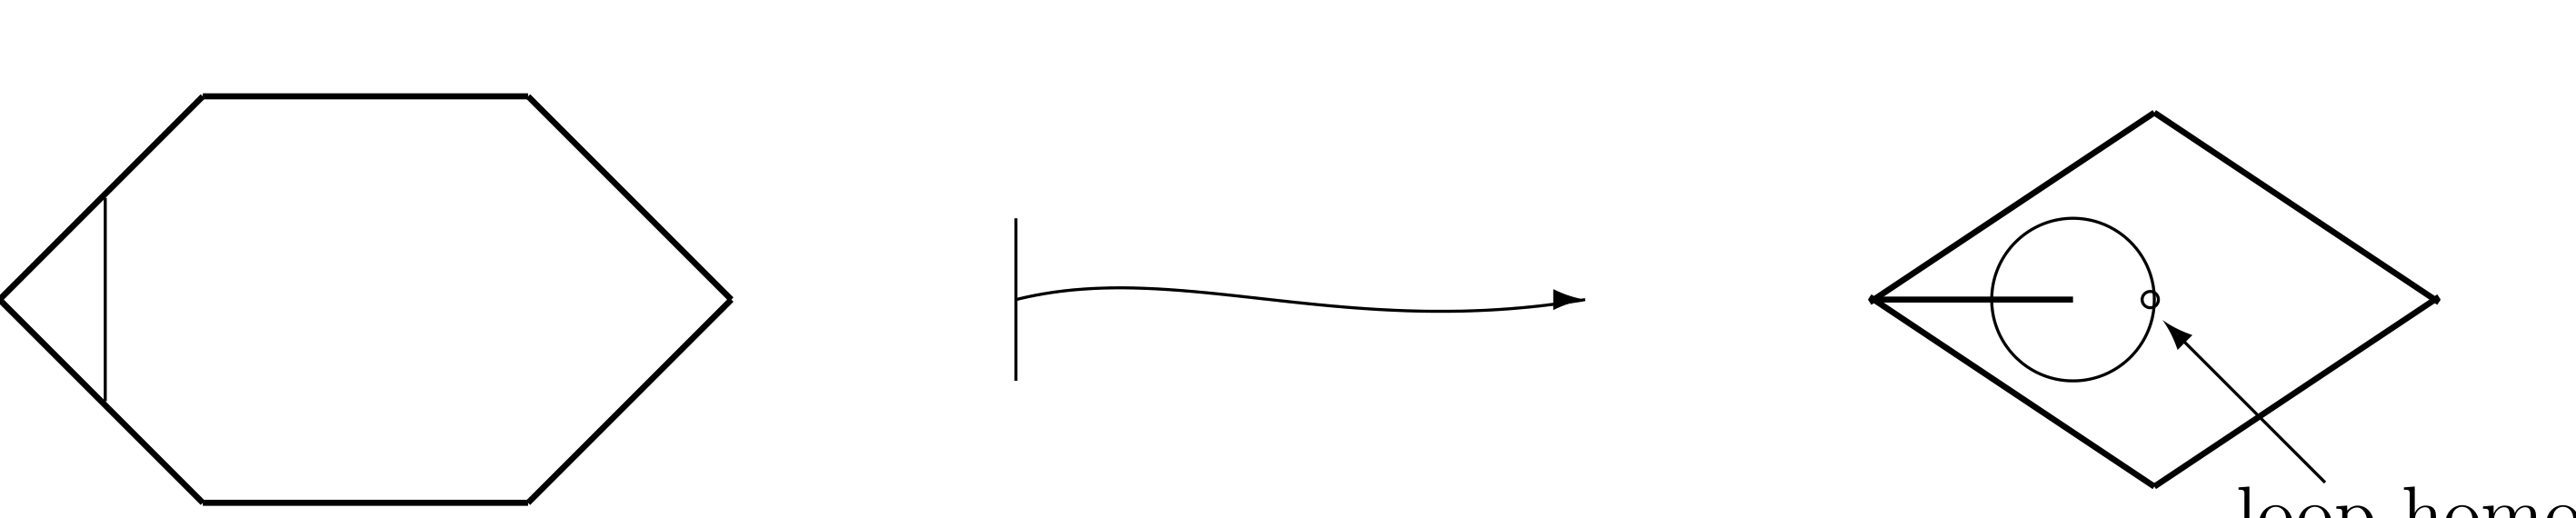
\includegraphics[width=12.0cm]{figures/fig-19.png}
  \caption{（原文无图题）\figorig{70}{19}}
  \label{fig:19}
\end{figure}


\begin{figure}[htbp]
  \centering
  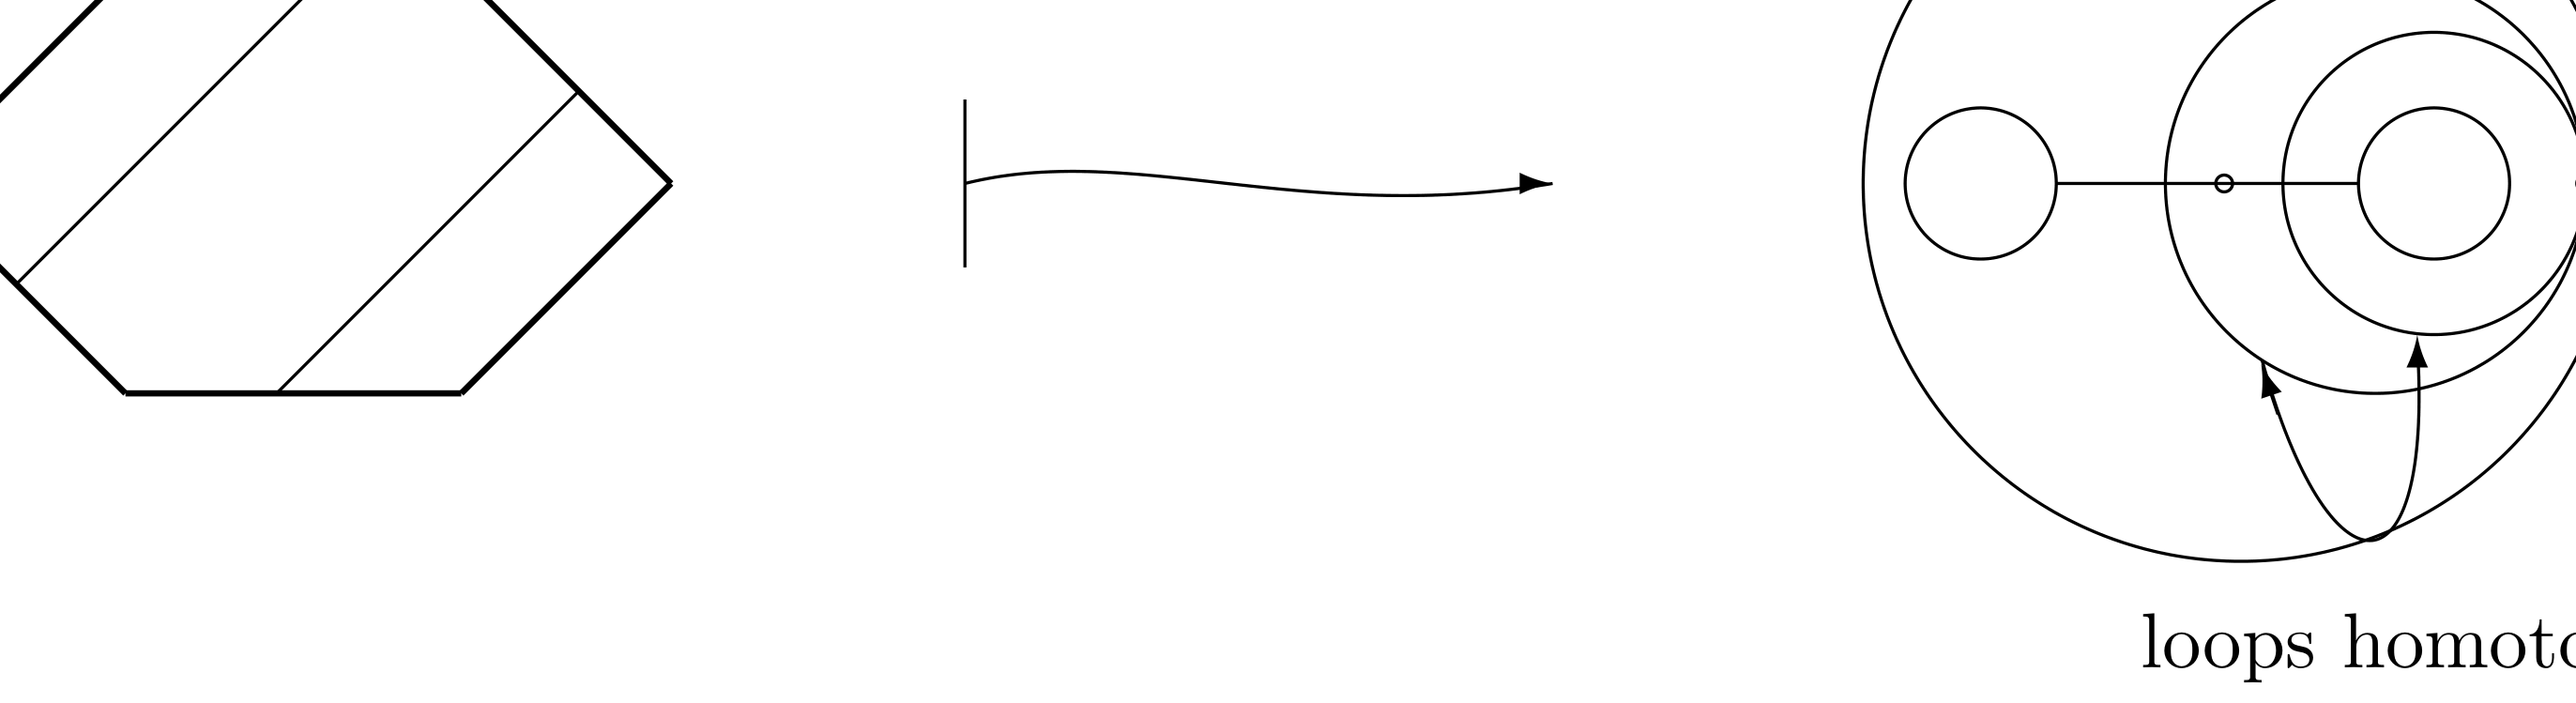
\includegraphics[width=11.62cm]{figures/fig-20.png}
  \caption{（原文无图题）\figorig{70}{20}}
  \label{fig:20}
\end{figure}


该引理在几何上显而易见，其证明只需画图（(i) 见图 19，(ii) 见图 20）。受该引理启发，我们也把 (i) 与 (ii) 中关于粘合的条件称为条件 (A) 与 (B)。

用 $\varepsilon_{\rm g}(n),\mu_{\rm g}(n),\lambda_{\rm g}(n)$ 分别表示把一个（带标号的）$2n$ 边形粘合成亏格为 ${\rm g}$ 的曲面的粘合数：分别不加任何条件、满足条件 (A)、满足条件 (A),(B)（因此 $\varepsilon_{\rm g}(n)$ 就是我们此前研究过的量）。

\begin{proposition} 有\footnote{注意对几乎所有的 $n$ 都有 $\lambda_{\rm g}(n)=0$，因此该和为有限和。}
$$
\chi(\Gamma_{\rm g}^1)=\sum_n (-1)^{n-1}\frac{\lambda_{\rm g}(n)}{2n}.
$$
\end{proposition}

\begin{proof}
每个填满弧系 $\sigma$ 来自 $2n/|{\rm Stab(\sigma)}|$ 个粘合（因为对所得的带弧系曲面而言，多边形的标号无关紧要）。于是结论由 Quillen 公式得出。
\end{proof}

\subsection{$\sum_n (-1)^{n-1}\frac{\lambda_{\rm g}(n)}{2n}$ 的计算}

现在只剩计算右端的和。为此需要把 $\lambda_{\rm g}(n)$ 与已经算出的 $\varepsilon_{\rm g}(n)$ 联系起来。这由下述引理完成。

\begin{lemma}\label{rel}
(i) 有
$$
\varepsilon_{\rm g}(n)=\sum_i \begin{pmatrix}2n\\ i\end{pmatrix}
\mu_{\rm g}(n-i).
$$
(ii) 有
$$
\mu_{\rm g}(n)=\sum_i \begin{pmatrix}n\\ i\end{pmatrix}
\lambda_{\rm g}(n-i).
$$
\end{lemma}

\begin{proof}(i) 设 $\sigma$ 是顶点带标号的 $2n$ 边形 $\Delta$ 的边的配对。若存在一对相邻的边被配对，就可以把它们互相粘合起来，得到 $2n-2$ 边形。如此尽可能地进行下去，最终得到 $2n-2i$ 边形 $\Delta_\sigma$ 及其边的一个满足条件 (A) 的配对 $\sigma'$。注意 $\Delta_\sigma$ 与 $\sigma'$ 不依赖于相邻边粘合的先后次序，并且 $\Delta_\sigma$ 有一个由“旧”标号递增顺序给出的标准标号 $1,...,2n-2i$。现在断言每个 $(\Delta_\sigma,\sigma')$ 恰好以 $\begin{pmatrix}2n\\ i\end{pmatrix}$ 种方式得到；这就给出所需结论。

事实上，考察 $\Delta$ 中最终落入 $\Delta_\sigma$ 内部的顶点。它们被映为内部的 $i$ 个点（每粘合一对边就产生一个新点）。称这些点为 $w_1,...,w_i$，并令 $\nu_j$ 为映到 $w_j$ 的 $\Delta$ 的顶点的最小标号（这里顶点标号使第 $k$ 条边连接顶点 $k$ 与顶点 $k+1$）。则 $\nu_1,...,\nu_i$ 是 $\lbrace{1,...,2n\rbrace}$ 的一个子集。在给定 $(\Delta_\sigma,\sigma')$ 时，这个子集完全决定了配对 $\sigma$：具体地说，应选出一个 $\nu_j$，使得对任意 $k$ 都有 $\nu_{j}+1\ne \nu_k$，然后把与 $\nu_j$ 相邻的两条边粘合；再把其余顶点按“旧”标号的递增顺序重新标为 $1,...,2n-2$，然后重复上述步骤，如此继续。由此也可看出，任何这样的 $\nu_j$ 集合都可能出现。这就证明了 (i)。

(ii) 设 $\sigma$ 是 $\Delta$（其边带标号）的配对，满足条件 (A)，但不必满足 (B)。若 $a_1,a_2$ 是相邻的边，且按相反顺序粘到相邻的边 $b_2,b_1$ 上，则可以把 $a_1,a_2$ 合并成一条边 $a$，把 $b_2,b_1$ 合并成 $b$，得到一个带配对的 $2n-2$ 边形。如此尽可能地进行下去，最终得到带新配对 $\sigma'$ 的 $2n-2i$ 边形 $\Delta_\sigma$，且该配对满足条件 (A) 与 (B)。在 $\Delta_\sigma$ 中，每一对（第 $j$ 对）边都是由 $\Delta$ 中的 $m_j+1$ 对边得到的。于是 $\sum_{j=1}^{n-i}m_j=i$。此外，对任意 $(\Delta_\sigma,\sigma')$，数集 $m_1,...,m_{n-i}$ 唯一确定了 $(\Delta,\sigma)$，只差确定构成 $\Delta_\sigma$ 第一条边的 $m_1+1$ 条边中哪一条应标为 1。因此每个 $(\Delta_\sigma,\sigma')$ 出现的次数由下述公式给出：
$$
\sum_{m_1,...,m_{n-i}:\sum_{j=1}^{n-i} m_j=i}(m_1+1).
$$
容易证明（请自行验证！）这个数等于 $\begin{pmatrix}n\\ i\end{pmatrix}$。这就证明了 (ii)。
\end{proof}

% [Tutor Note: 证明 (ii) 中“容易证明（请自行验证！）”掩盖了一个标准的组合恒等式：把 $i$ 分成 $n-i$ 个非负整数 $m_1,...,m_{n-i}$ 的有序分拆，求和 $\sum (m_1+1)$。其中分拆的个数为 $\binom{n-1}{i}$，而由对称性 $\sum m_1=\frac{i}{n-i}\binom{n-1}{i}=\binom{n-1}{i-1}$（各部分的地位对称，总和为 $i\binom{n-1}{i}$ 均摊到 $n-i$ 个位置），两者相加恰为 $\binom{n-1}{i}+\binom{n-1}{i-1}=\binom{n}{i}$。这就是 (ii) 中被略去的“一步”。]

定理 \ref{hz} 证明的完成现在依赖于下述计算引理。

\begin{lemma}\label{tech}
设 $\varepsilon(n),\mu(n),\lambda(n)$（$n\ge 0$）是满足方程
$$
\varepsilon(n)=\sum_i \begin{pmatrix}2n\\ i\end{pmatrix}
\mu(n-i);
$$
$$
\mu(n)=\sum_i \begin{pmatrix}n\\ i\end{pmatrix}
\lambda(n-i).
$$
的数列。并设 $\varepsilon(n)=\binom{2n}{
  n}f(n)$，其中 $f$ 是满足 $f(0)=0$ 的多项式。则 $\lambda(0)=0$，$\lambda(n)$ 只有有限多个非零值，且
$$
\sum_{n\ge 1} (-1)^{n-1}\frac{\lambda(n)}{2n}=f'(0).
$$
\end{lemma}

\begin{proof}
先考虑由引理中方程联系起来的任意数列 $\varepsilon(n)$、$\mu(n)$、$\lambda(n)$。设 $E(z)$、$M(z)$、$L(z)$ 为它们的生成函数（即 $E(z)=\sum_{n\ge 0}\varepsilon(n)z^n$ 等等）。我们断言
$$
E(z)=\frac{1+\sqrt{1-4z}}{2(1-4z)}L\left(\frac{1-\sqrt{1-4z}}{2\sqrt{1-4z}}\right).
$$
为看出这一点，只需考虑某个 $k$ 对应的情形 $\lambda_i=\delta_{ki}$。此时
$$
E(z)=\sum_{i,n}\begin{pmatrix} 2n\\ i\end{pmatrix}
\begin{pmatrix} n-i\\ k\end{pmatrix}z^n=
\sum_{p,q\ge 0}\begin{pmatrix} 2p+2q\\ p\end{pmatrix}
\begin{pmatrix} q\\ k\end{pmatrix}z^{p+q}.
$$
但函数
$$
F_r(z):=\sum_{p\ge 0}\begin{pmatrix} 2p+r\\ p\end{pmatrix}z^p
$$
等于
$$
F_r(z)=
\frac{1}{\sqrt{1-4z}}\biggl(\frac{1-\sqrt{1-4z}}{2z}\biggr)^r,
$$
这由递推
$$
F_r=z^{-1}(F_{r-1}-F_{r-2}),
$$
（$r\ge 2$）用归纳法容易看出。把它代入 $E(z)$ 的公式，经过平凡的化简即得
$$
E(z)=\frac{1+\sqrt{1-4z}}{2(1-4z)}\left(\frac{1-\sqrt{1-4z}}{2\sqrt{1-4z}}\right)^k,
$$
正是所要求的。

现在假设 $\varepsilon(n)$ 满足多项式性条件。这意味着 $E(z)=P(z\partial)|_{z=0}\frac{1}{\sqrt{1-4z}}$，其中 $P$ 是常数项为零的多项式。为证明我们的断言，只需考虑情形 $P(z)=(1+a)^z-1$，其中 $a$ 是形式参数（于是 $P'(0)=\log(1+a)$）；事实上该形式级数的系数是 $\binom{z}{j}$（$j\ge 1$），它们在常数项为零的 $z$ 的多项式空间中构成一组基。此时得到
$$
E(z)=\frac{1}{\sqrt{1-4(1+a)z}}-\frac{1}{\sqrt{1-4z}}.
$$
因此
$$
L(u)=\frac{1}{1+u}\left(\frac{1}{\sqrt{1-4au(1+u)}}-1\right).
$$
从而
$$
\sum_k (-1)^{k-1}\frac{\lambda_k}{2k}=\frac{1}{2}\int_{-1}^0 L(u)\frac{du}{u}=
\frac{1}{2}\sum_{p\ge 1} \begin{pmatrix} 2p\\ p\end{pmatrix}
(-1)^{p-1}a^p\int_0^1x^{p-1}(1-x)^{p-1}dx.
$$
但 $\int_0^1x^{p-1}(1-x)^{p-1}dx$ 是 欧拉 Beta 积分，等于 $\frac{(p-1)!^2}{(2p-1)!}$。于是
$$
\sum_k (-1)^{k-1}\frac{\lambda_k}{2k}=\sum_{p\ge 1}(-1)^{p-1}\frac{a^p}{p}=\log(1+a),
$$
正是所要求的。
\end{proof}

% [Tutor Note: 这里的“平凡的化简”掩盖了两个关键代换。第一，令 $u=\frac{1-\sqrt{1-4z}}{2\sqrt{1-4z}}$，则 $\sqrt{1-4z}=1/(1+2u)$，等价于 $z=\frac{u(1+u)}{(1+2u)^2}$（而非 $z=-u/(1+u)^2$；可用 $z=0.01$ 时 $u\approx0.0103$ 作数值核对）。于是 $L$ 的级数被拉回到 $u$ 的级数；$E(z)$ 的平方根结构正好对应这个代换（属于 Lagrange 反演的标准手法）。第二，由 $L(u)/u=\sum_{p\ge1}\binom{2p}{p}a^p u^{p-1}(1+u)^{p-1}$，作 $u=-x$ 逐项积分得 $\int_{-1}^0 L(u)du/u=\sum_p(-1)^{p-1}\binom{2p}{p}a^p B(p,p)$（若要写成 $(0,\infty)$ 上的 Beta 积分，则应作 $u=-x/(1+x)$，此时 $\int_0^\infty x^{p-1}/(1+x)^{2p}dx=B(p,p)$），再配合 $\frac12\binom{2p}{p}B(p,p)=\frac1p$，才得到 $\sum_p(-1)^{p-1}a^p/p=\log(1+a)$。若直接用 $u$ 的级数逐项积分，会漏掉这一 Beta 积分表示。]

\subsection{定理 \ref{hz} 证明的完成}

现在来完成 Harer–Zagier 定理的证明。回忆我们用矩阵积分证明了公式
\begin{equation}\label{Pn}
P_n(x):=\sum_{\rm g} \varepsilon_{\rm g}(n)x^{n+1-2{\rm g}}
=\frac{(2n)!}{2^nn!}\sum_{p\ge 0}\begin{pmatrix} n\\ p\end{pmatrix}
2^p\begin{pmatrix} x\\ p+1\end{pmatrix}.
\end{equation}

令 $q:=n-p$。则表达式 (\ref{Pn}) 化为
\begin{equation}\label{Pn1}
P_n(x)=\begin{pmatrix} 2n\\ n\end{pmatrix}
\sum_{q\ge 0}2^{-q}\begin{pmatrix} n\\ q\end{pmatrix}\frac{n!}{(n-q+1)!}
x(x-1)...(x-n+q).
\end{equation}

现在断言：多项式 $\frac{P_n(x)}{x^{n+1}}$ 中 $x^{-2{\rm g}}$（${\rm g}\ge 1$）的系数形如 $\binom{2n}{n}f_{\rm g}(n)$，其中 $f_{\rm g}$ 是多项式。事实上，对 $x^{-2{\rm g}}$ 系数的贡献只来自 $q\le 2{\rm g}$ 的项，因此只需验证每一项贡献都具有上述形式。这归结为验证 Laurent 多项式 $Q(x,n)=(1-\frac{1}{x})...(1-\frac{n}{x})$ 的系数是 $n$ 的多项式，且在 $-1$ 处取零（当然，首项系数除外）。为看出这一点，令 $Q(x,a)=\frac{\Gamma(x)}{\Gamma(x-a)x^a}$（当 $a=n$ 时它等于 $Q(x,n)$）。该函数在 $x\to +\infty$ 时有关于 $\frac{1}{x}$ 的渐近 Taylor 展开，它可由公式 \eqref{stir} 给出的 $\Gamma(x)$ 的 Stirling 渐近展开得到，并且容易证明其系数是 $a$ 的多项式。此外 $Q(x,-1)=1$，由此即得所需结论。

此外断言 $f_{\rm g}(0)=0$：这同样来自 $Q(x,a)$ 展开式的非首项系数在 $a=0$ 处取零这一事实。而这是显然的，因为 $Q(x,0)=1$。

于是我们处于可以应用引理 \ref{tech} 的情形。因此只剩计算 $\sum_{{\rm g}\ge 1}f_{\rm g}'(0)x^{-2{\rm g}}$。为此注意 $q>1$ 的项对 $f_{\rm g}'(0)$ 没有贡献，因为它们给出的 $n$ 的多项式都被 $n^2$ 整除。所以只需考虑 $q=0$ 与 $q=1$。对 $q=1$，贡献是
$$
\tfrac{1}{2x}(1-\tfrac{1}{x})...(1-\tfrac{n}{x})
$$
在 $n=0$ 处的值，即 $\frac{1}{2x}$。对 $q=0$，贡献是 $\frac{1}{n+1}(1-\frac{1}{x})...(1-\frac{n}{x})$ 对 $n$ 在 $0$ 处的导数，即
$$
\tfrac{d}{da}|_{a=0}\tfrac{Q(x,a)}{a+1}=-1+\tfrac{d}{da}|_{a=0}Q(x,a).
$$
因此（渐近地）有
$$
\sum_{{\rm g}\ge 1}f_{\rm g}'(0)x^{-2{\rm g}}=\tfrac{1}{2x}+\tfrac{d}{da}|_{a=0}Q(x,a)=
\tfrac{1}{2x}+\tfrac{\Gamma'(x)}{\Gamma(x)}-\log x
$$
现在，由 \eqref{loggapri} 给出的 $\Gamma'/\Gamma$ 的渐近展开可知 $f_{\rm g}'(0)=-\frac{B_{2{\rm g}}}{2{\rm g}}$。这就完成了证明。

% [Tutor Note: 最后一步的符号值得核对：Stirling 展开给出 $\frac{\Gamma'(x)}{\Gamma(x)}=\log x-\frac{1}{2x}-\sum_{{\rm g}\ge 1}\frac{B_{2{\rm g}}}{2{\rm g}}x^{-2{\rm g}}+\dots$（即 $\psi(x)$ 的渐近式）。于是 $\frac{1}{2x}+\frac{\Gamma'(x)}{\Gamma(x)}-\log x=-\sum_{{\rm g}\ge 1}\frac{B_{2{\rm g}}}{2{\rm g}}x^{-2{\rm g}}$，右端的 $1/(2x)$ 恰好与 $\psi$ 展开中的 $-1/(2x)$ 抵消，剩下的正是 $-\frac{B_{2{\rm g}}}{2{\rm g}}$ 项。这解释了为何 $f_{\rm g}'(0)$ 带负号，也与定理 \ref{hz} 中 $\chi(\Gamma_{\rm g}^1)=-\frac{B_{2{\rm g}}}{2{\rm g}}$ 的符号一致；注意 $B_{2{\rm g}}$ 本身对 ${\rm g}\ge 1$ 是正负交替的（$B_2=1/6,\ B_4=-1/30,\dots$）。]

\begin{exercise} 对 ${\rm g}=1$ 证明定理 \ref{mum}。
\end{exercise}

\begin{exercise}
设 $\Gamma(N)$ 是 $SL_2(\Bbb Z)$ 的同余子群，由模 $N$ 等于 $1$ 的矩阵组成。

(a) 证明当 $N\ge 3$ 时 $\Gamma(N)$ 是自由群。（提示：考虑 $\Gamma(N)$ 在上半平面上的作用。）并证明 $\Gamma(2)$ 是两个生成元上的自由群 $\Gamma_+(2)$ 与 $\Bbb Z/2\Bbb Z$ 的直积。

(b) 求 $\Gamma(N)$（$N\ge 3$）的无关系生成元的个数。（提示：计算 $\chi(\Gamma(N))$。）
\end{exercise}

\begin{exercise} 设 $\Gamma$ 是由生成元 $a,b,c$ 及定义关系 $ab=ba$ 定义的群。求 $\Gamma$ 的欧拉示性数。
\end{exercise}

\begin{exercise} 考虑双曲平面 $H=\Bbb C_+$ 中内角为 $\alpha=\frac{\pi}{2}$、$\beta=\frac{\pi}{3}$、$\gamma=\frac{\pi}{7}$ 的三角形 $\Delta$，并令 $\Gamma$ 为 $PSL_2(\Bbb R)$ 中由绕 $\Delta$ 各顶点分别旋转 $2\alpha,2\beta,2\gamma$ 的旋转 $a,b,c$ 生成的子群。

(i) 证明 $H/\Gamma$ 自然同胚于由两份 $\Delta$ 粘成的球面，可视为带有三个非平凡稳定子点（阶分别为 2、3、7）的轨形。

(ii) 计算欧拉示性数 $\chi(\Gamma)$。

(iii) 证明 $\Gamma$ 的定义关系为
$$
a^2=1,\ b^3=1,\ c^7=1,\ abc=1
$$
（利用 van Kampen 定理的轨形版本）。

(iv) 构造满同态 $\phi: \Gamma\to PSL_2(\Bbb F_7)$。

(v) 证明 ${\rm Ker}\phi$ 无挠，且 $H/{\rm Ker}\phi$ 是亏格为 $3$ 的紧 Riemann 曲面 $X$，带有 $PSL_2(\Bbb F_7)$ 的作用。把 $X$ 等同于 $\Bbb C\Bbb P^2$ 中的 Klein 四次曲线 $x^3y+y^3z+z^3x=0$。
\end{exercise}

\bigskip
\noindent\rule{\textwidth}{0.6pt}

